\documentclass[12pt,a4paper]{article}
%\usepackage{cmap}
%\usepackage[T1, T2A]{fontenc}
\usepackage[utf8]{inputenc}
\usepackage[russian]{babel}
\usepackage{amsmath,amssymb}
\usepackage{parskip}
\usepackage{caption}
\usepackage{textcomp}
\usepackage{gensymb}
\usepackage[dvips]{graphicx}
\usepackage{wrapfig}
\usepackage{color}
\usepackage{setspace}
%\usepackage{hyperref}
\usepackage{epstopdf}

\oddsidemargin=-0.5 cm
\evensidemargin=-0.5 cm
\textwidth=170 mm
\textheight=260 mm
\topmargin=0 cm
\voffset= -2cm
\pagenumbering{false}
%\newlength{\varheight}
%\setlength{\varheight}{3.1cm}
\setlength{\parindent}{0cm}
\spacing{1.1}
\parskip=2mm
\clubpenalty=10000
\widowpenalty=10000

\begin{document}

Из уравнений движения малых участков веревки в проекции на оси координат
$$
  \left\{
  \begin{aligned}
  \mu gdl&=-d(T\cos\alpha),\\
  \mu\omega^2 xdl&=-d(T\sin\alpha).
  \end{aligned}
  \right.
$$
Здесь $\mu$ --- масса единицы длины веревки, $T$ --- сила ее натяжения.

\begin{figure}[!h]
\begin{center}
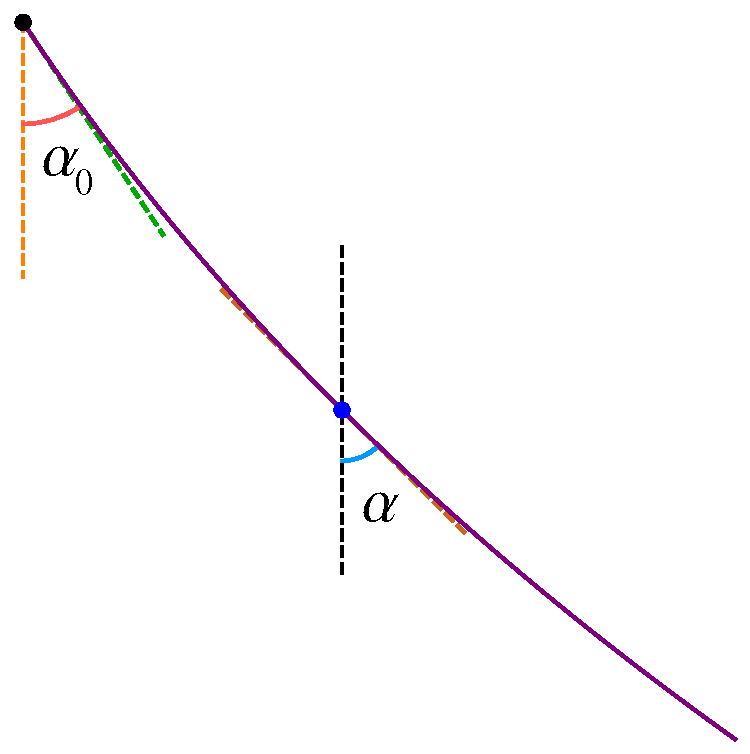
\includegraphics[scale=0.7]{ropeangle.pdf}
\end{center}
\end{figure}

Параметризуем все неизвестные величины переменной $\lambda=l/L$, где $l$ --- криволинейная координата, отсчитанная вдоль веревки, $L$ --- длина веревки. Исключим натяжение $T$ и введем переменную $t(\lambda)=\tan\alpha$. Тогда уравнение запишется в виде
$$
  (1-\lambda)t''-2t'+\frac{at}{\sqrt{1+t^2}}=0,
$$
где $a=\omega^2 L/g$, а производная берется по $\lambda$. Уравнение можно упростить заменой $z=(1-\lambda)t$:
$$
  z''+\frac{az}{\sqrt{(1-\lambda)^2+z^2}}=0.
$$
Самое интересное только начинается. Определим начальные условия задачи. Интегрируя первое уравнение движения (вдоль оси $Oy$), получим
$$
  \mu gl=T_0 \cos\alpha_0-T\cos\alpha,
$$
где $T_0$ --- натяжение в точке крепления. Подставляя это во второе уравнение движения при $l=x=0$ (точка крепления), получим одно ``начальное'' условие $t'(0)=t(0)$. Второе начальное условие записать довольно сложно в терминах величины $t$, оно утверждает, что натяжение в конце веревки равно нулю. В интегральной форме оно имеет вид
$$
  t(1)=a\int\limits_0^1 \frac{td\lambda}{\sqrt{1+t^2}}.  
$$
Гораздо проще \textit{сформулировать} эти начальные условия для переменной $z$. Из первого условия на $t$ получим $z'(0)=0$. Так как $t(1)$ конечна, то из второго условия получим
$$
  z(1)=0.
$$
Вот здесь проблемка. Ведь просто подставить $z(1)=0$ не получится ввиду расходимости.. [на самом деле расходимости там не должно быть, но ее надо устранять ручками]

Но это еще не самое главное. Мне с трудом, но все же удалось просчитать численно форму веревки.
\begin{figure}[!h]
\begin{center}
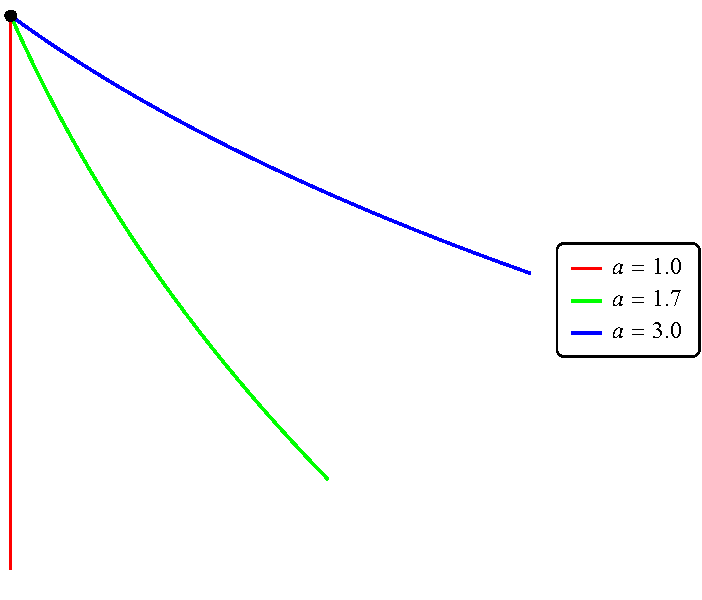
\includegraphics[scale=1]{ropeshape.pdf}
\end{center}
\end{figure}

Результат оказался довольно интересным. При небольших $a$, например $a=1$, веревка висела камнем вниз. При больших же значениях угловой скорости, скажем $a=3$, она таки замечала вращение и отклонялась. Теперь внимание, вопрос: какое такое критическое значение $a$, при котором вертикальное положение веревки перестает быть единственным равновесным? Предположительно, что оно еще и перестает быть устойчивым при этом значении $a$, но это уже гипотезы.

\end{document}

